\subsection{Reserved results and loop coverage}
\label{sec:general-results}
The corrected shared model completes 43 matched nontrivial requests from the 110-request grid. The coverage record contains 21 failed reference calculations, 10 failed enlarged-region checks, 0 incomplete method comparisons, and 36 inputs above the native coordinate limit. Identity-only batches number 0. The matched outputs pass 5,976 coefficient comparisons. Table~\ref{tab:general-coverage} retains every loop order and outcome.

Complete supplied-basis time, summed over request medians, is 63.450 seconds for native choices, 60.094 seconds for the common fixed setting, 57.125 seconds for the shared model, and 59.198 seconds for the preceding application. The learned-to-native ratio is 0.900, with repeat interval [0.867,0.919]. The learned-to-fixed ratio is 0.951, with interval [0.916,0.971]. Relative to the preceding application, the ratio is 0.965, with interval [0.900,0.979]. All ratios include inference, checking, and recovery.

The 15 matched requests from excluded families or higher orders give a learned-to-native ratio of 0.939, with repeat interval [0.897,0.978], and a learned-to-fixed ratio of 0.885, with interval [0.840,0.927]. Their physical groups were excluded from both fitting and model selection.

\begin{table}[!htbp]\centering\small
\caption{The shared model across physical classes. Ratios use sums of median times on each matched set. Values below one mean less complete time. A class can contain both training-domain and held-out loop orders.}
\label{tab:general-classes}
\begin{tabularx}{\linewidth}{@{}Yrrr@{}}\toprule
Physical class & Matched & Model/native & Model/fixed\\\midrule
Box with bubbles & 4 & 0.597 & 0.981\\
Four-point ladder & 4 & 1.109 & 1.042\\
Nonplanar box & 1 & 1.040 & 1.010\\
Box with a virtual leg & 2 & 1.092 & 0.965\\
Pentagon & 2 & 0.977 & 0.915\\
Massive two-point & 7 & 0.957 & 0.898\\
Massless two-point & 7 & 0.793 & 0.988\\
Distinct-mass vacuum & 7 & 0.861 & 0.812\\
One-mass vacuum & 9 & 1.140 & 0.983\\
\bottomrule\end{tabularx}\end{table}

The model changes the initial action from native bounds on 43 matched requests and from the fixed control on 17. Thus the comparison records actual action changes as well as complete time. Reference discovery across the requested grid takes 1056.4 seconds and the independent checks take 772.2 seconds, including unsuccessful attempts. These costs precede the matched supplied-basis timings. The new fit takes 9.5 seconds and reuses the existing cost labels; this fitting time does not include the earlier cost of generating those labels.

\begin{table}[!htbp]\centering\small
\caption{Every requested loop order in the corrected-model test. ``Reference'' includes failed initial or enlarged-region reductions. ``Method'' means an incomplete matched comparison. A dash means that no complete ratio is available. The last column compares the shared model with native choices on matched nontrivial requests.}
\label{tab:general-coverage}
\begin{tabular}{@{}rrrrrrr@{}}\toprule
Loops & Requests & Matched & Reference & Method & Unsupported & Ratio\\\midrule
1 & 12 & 12 & 0 & 0 & 0 & 1.027\\
2 & 14 & 13 & 1 & 0 & 0 & 0.990\\
3 & 12 & 10 & 2 & 0 & 0 & 0.712\\
4 & 12 & 6 & 6 & 0 & 0 & 0.827\\
5 & 12 & 2 & 10 & 0 & 0 & 1.172\\
6 & 10 & 0 & 8 & 0 & 2 & ---\\
7 & 8 & 0 & 4 & 0 & 4 & ---\\
8 & 6 & 0 & 0 & 0 & 6 & ---\\
9 & 6 & 0 & 0 & 0 & 6 & ---\\
10 & 6 & 0 & 0 & 0 & 6 & ---\\
11 & 6 & 0 & 0 & 0 & 6 & ---\\
12 & 6 & 0 & 0 & 0 & 6 & ---\\
\bottomrule\end{tabular}\end{table}
\begin{figure}[!htbp]\centering
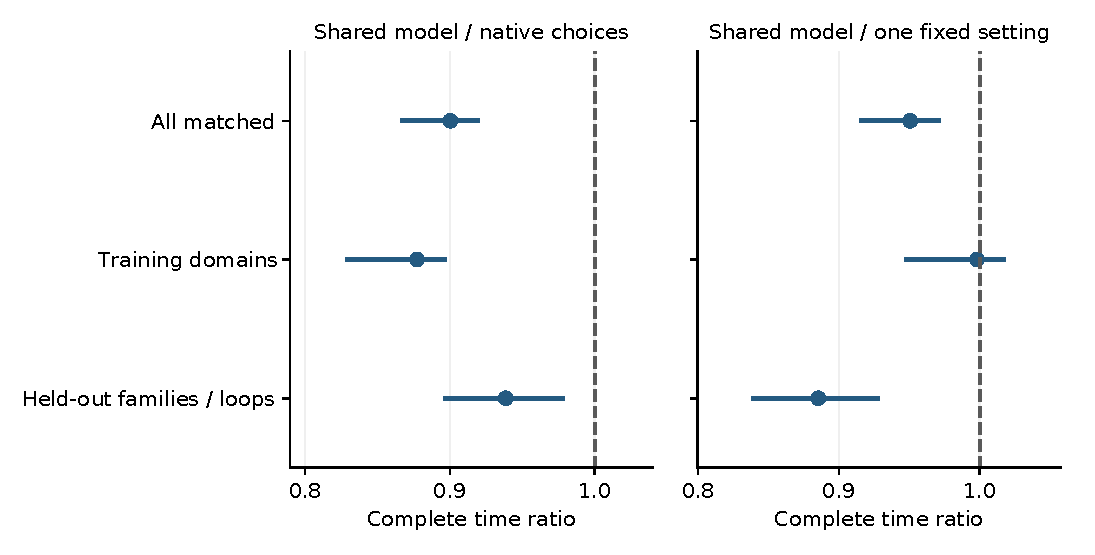
\includegraphics[width=\linewidth]{paper_figures/general_policy_times.pdf}
\caption{Complete time of the corrected shared model, separated into training domains and physical holdouts. Both controls use the same exact implementation. The fixed control has one setting for all requests. The line at one marks equal time, and the intervals describe paired repeat variation.}
\label{fig:general-times}
\end{figure}
\begin{figure}[!htbp]\centering
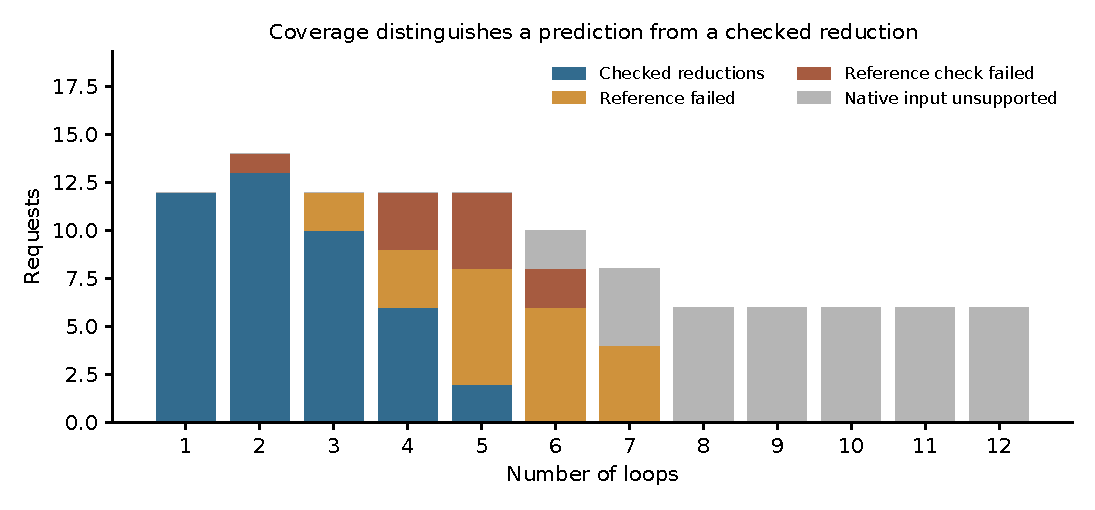
\includegraphics[width=\linewidth]{paper_figures/general_policy_coverage.pdf}
\caption{The loop range extends through twelve, while native completion has a smaller measured range. Predictions for unsupported inputs do not count as reductions. Failed reference checks also prevent a timing claim.}
\label{fig:general-coverage}
\end{figure}
\FloatBarrier
The family holdouts test transfer within this finite set of denominator structures, target powers, and rational parameter values. They do not establish performance for arbitrary graph routings, large target ranks, general symbolic kinematics, cuts, or unbounded loop order. The same physical definitions have also been used in earlier project development, although the excluded groups supply no labels or model-selection costs to this new fit. The high-loop failures and native input limits therefore remain part of the result.
